%!TEX root = ./main.tex
\section{Static Approach}
\label{sec:ruleDerivation}

As discussed in the overview, some syntactic sugar may appear multiple times in one evaluation, and it is extremely cumbersome to derive it in CoreLang. This will make the evaluation of this syntactic sugar very inefficient. If we can statically analyze its evaluation rules through the structure of syntactic sugar, this will greatly improve the efficiency of syntactic sugar. In this section, we will give one such method to make resugaring of syntactic sugar more efficient.
\todo{@ziyi: sugars; 'extremely' too strong?; derive -> desugar? ; If..., it will.; such a}

Considering a simple syntactic sugar
\[\drule{(\m{not}~e_1)}{(\m{if}~e_1~\m{\#f}~\m{\#t})},\]
we expect to get the evaluation rules of \m{not}. In fact, we need to \textit{embed} the evaluation rules of \m{if}. So we need a method that can express evaluation rules and is easy to transform. To accomplish these goals, we designed \textit{inference automaton} (IFA), which can be visually described by graphs. Readers do not need to know the definition of IFA now, we will discuss it later.

Assuming that we already know the IFA of all syntactic structures in CoreLang, the method of using IFA to construct the evaluation rules of syntactic sugar is as follows: First, construct the IFA of syntactic sugar according to the desugar rules and IFA of CoreLang. Then, transform and simplify IFA. Finally, generate evaluation rules for syntactic sugar.
\todo{@ziyi: IFAs?}

In this section, we first give some examples of IFA and its formal definition. Then we will discuss a more strict IFA called standard IFA, which deformed by IFA. Next, we give the algorithm of conversion between evaluation rules and IFA. Finally, we discuss the role of IFA in dealing with syntactic sugar.

\subsection{Inference Automaton}

As mentioned above, IFA intuitively describes the evaluation rules of a certain syntactic structure. To help readers better understand it, first we give some examples, then we give the formal definition of IFA.
\todo{@ziyi: 'first give' may be replaced by 'start with' to avoid duplicate 'give'}

\subsubsection{IFA of if}

The evaluation rules of \texttt{if} are shown as belows.
\todo{@ziyi: follows}

\infrule[E-If]{e_1 \to e_1'}{(\m{if}~e_1~e_2~e_3) \to (\m{if}~e_1'~e_2'~e_3')}
\infax[E-IfTrue]{(\m{if}~\m{\#t}~e_2~e_3) \to e_2}
\infax[E-IfFalse]{(\m{if}~\m{\#f}~e_2~e_3) \to e_3}
We can observe that a term with \m{if} is first evaluated for $e_1$, and is chosen to be evaluated for $e_2$ or $e_3$ depending on the value of $e_1$. Then the result of the evaluation of $e_2$ or $e_3$ is the value of the term. Thus, we use Figure \ref{fig:ifa-if} to represent the evaluation rules of \m{if}.
\todo{@ziyi :headed with, e2' 's superscript? }

\begin{figure}[t]
	\centering
	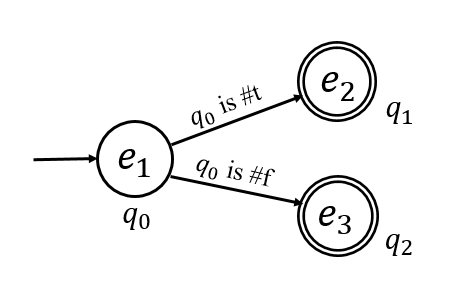
\includegraphics[scale=0.3]{images/ifa-if.png}
	\caption{IFA of \m{if}}
	\label{fig:ifa-if}
\end{figure}

A node of IFA indicates that this item needs to be evaluated, and the node before this has been evaluated. The arrow from $q_0$ to $q_1$ indicate that this branch will be selected when the evaluation result of $e_1$ is \m{\#t}. The arrow between $e_1$ and $e_3$ is similar. The double circles of $e_2$ and $e_3$ denotes that their evaluation result is the result of the term with this syntactic structure. When a term with an \m{if} syntactic structure needs to be evaluated (for example \m{(if (if \#t \#t \#f) \#f \#t)}), first evaluating the $e_1$ (\m{(if \#t \#t \#f)}). Note that in this process, evaluating a subexpression requires running another automaton based on its syntax, while the outer automaton hold the state at $q_0$. According to the result of $e_1$ (\m{\#f}), the IFA selects the branch ($e_3$). Then the result of $e_3$ (\m{\#t}) will be the evaluation result of the term.
\todo{@ziyi: indicates; denote; the result of their own?}

\subsubsection{IFA of nand}

Sometimes the rules may be more complex, such as being reduced into another syntactic structure, or a term containing other syntactic structures. For example, we can express nand's evaluation rules as follows. Based on the method discussed above, we can draw nand's IFA as Figure \ref{fig:ifa-nand-a}.

\infrule[E-Nand]{e_1 \to e_1'}{(\m{nand}~e_1~e_2) \to (\m{nand}~e_1'~e_2)}
\infax[E-NandV]{(\m{nand}~v_1~e_2) \to (\m{if}~(\m{if}~v_1~e_2~\m{\#f})~\m{\#f}~\m{\#t})}


\begin{figure}[thbp]
\centering
\subcaptionbox{IFA obtained directly according to the original rules \label{fig:ifa-nand-a}}[.4\linewidth]{
    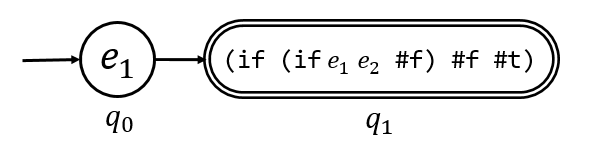
\includegraphics[scale=0.25]{images/ifa-nand-1.png}
}
\subcaptionbox{After expanding the outer \m{if} \label{fig:ifa-nand-b}}[.4\linewidth]{
    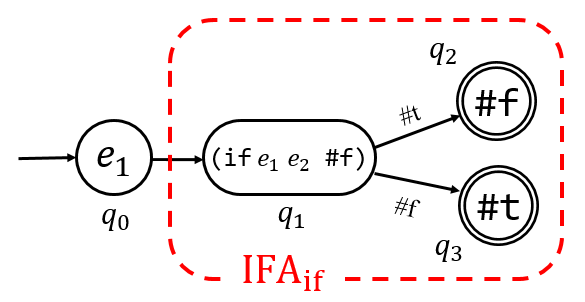
\includegraphics[scale=0.25]{images/ifa-nand-2.png}
}
\subcaptionbox{After expanding the inner \m{if} \label{fig:ifa-nand-c}}[.8\linewidth]{
    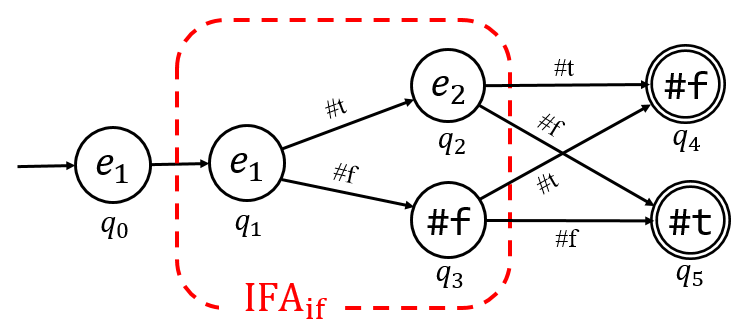
\includegraphics[scale=0.25]{images/ifa-nand-3.png}
}
\caption{IFA of \m{nand}}
\label{fig:ifa-nand}
\end{figure}

When the automaton runs to the terminal node of Figure \ref{fig:ifa-nand-a}, it will derive the \m{if} term. In fact, we have known how \m{if} works through the IFA of \m{if}. Thus we can replace the last node with an $\text{IFA}\_\m{if}$ and substitute $e_1$ to $e_3$ of $\text{IFA}\_\m{if}$ with the parameters of the node. Use the termination nodes of $\text{IFA}\_\m{if}$ as the termination nodes of the $\text{IFA}\_\m{nand}$. The results are shown in Figure \ref{fig:ifa-nand-b}. Further decomposing the inner nodes, connecting the terminating node of $\text{IFA}\_\m{nand}$ to the node pointed to by the original output edge, we get Figure \ref{fig:ifa-nand-c}.

As can be seen, the nodes of IFA in Figure \ref{fig:ifa-nand-c} have no other composite syntactic structures. Such an IFA completely expresses the semantics of a syntactic structure, and no longer cares about the evaluation rules of other syntactic structures. In fact, we will do the same steps for syntactic sugar to get IFA, which will be discussed later.

\subsubsection{IFA of or}

We represent the evaluation rule of or in a more complex way, as follows.

\infrule[E-Or]{e_1 \to e_1'}{(\m{or}~e_1~e_2) \to (\m{or}~e_1'~e_2)}
\infax[E-OrV]{(\m{or}~v_1~e_2) \to (\m{let}~x~v_1~(\m{if}~x~x~e_2))}
\todo{Whether the let expression is right? @ziyi }In this case, we use the let binding, which expresses a class of rules containing substitution. At this point, we need to record the term represented by each variable at each node, denoted by Γ. The representation of IFA\_or is shown in AAAP5.`

\subsubsection{Definition of IFA}

\begin{Def}[Inference Automaton]

An inference automaton (IFA) of syntactic structure \m{CoreHead} is a 5-tuple, $(Q, \Sigma, q_0, F, \delta)$, consisting of

\begin{itemize}
    \item A finite set of nodes $Q$, each node contains a expression and a symbol table. The expression can be a term or a pattern variable. The symbol table maps a variable to a node.
    \item A finite set of conditions $\Sigma$
    \item A start node $q_0 \in Q$
    \item A set of terminal nodes $F \subseteq Q$
    \item A transition function $\delta: (Q-F) \times \Sigma' \to Q$ where $\Sigma' \subseteq \Sigma$
\end{itemize}


and for each node $q$, there is no sequence of pattern $P = (p_1,p_2,\ldots,p_n)\subseteq \Sigma^*$, which makes that after $q$ transfers sequentially according to $P$, it returns $q$.

\end{Def}

The last constraint requires that there be no circles in our IFA.
\todo{@ziyi: constraint to restrict?}

In IFA, state transition does not depend on input. The only input IFA accepts is the term to be evaluated with this syntactic structure. The state transition is through pattern matching on the evaluation result of the term in the previous node. Note that IFA is associated with syntactic structure. At Each IFA only represents the current evaluation of a syntactic structure. The state indicates that some
sub-expressions of the syntactic structure have been evaluated, and the rest have not.
\todo{@ziyi: miss some articles?; each}

\subsection{Standard IFA}

Although IFA can intuitively show the behavior of a syntactic structure for evaluation, IFA itself has a complicated form. For example, the IFA of a syntactic structure may contain other syntactic structures. We expect stricter constraints on IFA to ensure that it has been analyzed and deformed.

\begin{Def}[Standard IFA]
\label{def:stdifa}
If an IFA meets following constraints, we call it a standard IFA.
\begin{itemize}
    \item The expression of node in $Q$ can only be $e_i$, a value or a pattern variable.
    \item For any $q_1,q_2 \in Q$ and $c_1, c_2 \in \Sigma$, $\delta(q_1, c_1) \neq \delta(q_2, c_2)$.
    \item On each branch,
\end{itemize}
\end{Def}

If an IFA is standard, it means there are no more composite syntactic structures in it. In the above example, for the syntactic structure of \m{if}, we substituted the IFA of the \m{if} into \m{nand} and converted it into a standard IFA. Below we will prove that it is always feasible to convert IFA to standard IFA, and give the algorithm.

\begin{mythm}[Standardizability of IFA]
\label{mythm:stdifa}
Considering an IFA of a syntactic structure, if the standard IFAs of all syntactic structures of terms contained in the IFA are known, then the IFA can be transformed into a standard IFA.
\end{mythm}



Before talking about standard IFA, we prove some properties of IFA.

\begin{lemma}[Splittablity]
\label{lemma:splittablity}
In an IFA $M$, if $\delta(q_1, c_1)=q$ and $\delta(q_2, c_2)=q$, we can build a new node $q'$, whose expression and symbol table are the same as $q$. Let $\delta(q_2, c_2)=q'$. If $q \in F$, let $q' \in F$. Otherwise, for each $c_i$ and $q_i$ that satisfy $\delta(q, c_i)=q_i$, let $\delta(q', c_i)=q_i$. We build a new IFA $N$ in this way. Then $N$ is equivalent to $M$.
\end{lemma}

\begin{lemma}[]

\end{lemma}





\begin{proof}[Proof of Theorem \ref{mythm:stdifa}]

\end{proof}

%===========================================
\subsection{Convert evaluation rules to IFA}

In the examples at the beginning of this section, we construct IFAs based on their semantics. Now, we will give an algorithm that can automatically convert the evaluation rules to IFA and ensure its correctness. But at the same time, it has stricter requirements on the evaluation rules.

\begin{Asm}
\label{Asm:rules}
A syntactic structure $CoreHead$ only contains the following evaluation rules.

\infrule[E-Head]
{e_i \to e_i'}
{(\m{CoreHead}~v_1\ldots v_p~e_1 \ldots e_i \ldots e_q) \to   (\m{CoreHead}~v_1\ldots v_p~e_1 \ldots e_i' \ldots e_q)}
\infax[E-HeadR] {(\m{CoreHead}~v_1 \ldots v_p~e_1 \ldots e_q) \to e}

\end{Asm}

This assumption specifies the form of the evaluation rules to ensure that IFAs can be generated. The first one is context rule, and the other one is reduction rule. $e$ could be any value, one of the parameters or a term of another syntactic structure.
\todo{@ziyi: a .. rule, could to can?}

\begin{Asm}[Orderliness of Syntactic Structure]
\label{Asm:orderliness}
The syntactic structure in CoreLang is finite. Think of all syntactic structures as points in a directed graph. If one of $CoreHead$'s evaluation rules can generate a term containing $CoreHead'$, then construct an edge that points from $CoreHead$ to $CoreHead'$. The directed graph generated in this method has no circles.
\end{Asm}

IFAs are not able to construct syntactic structures that contain recursive rules. This assumption qualifies that we can find an order for all syntactic structures, and when we construct IFA of $CoreHead$, IFA of $CoreHead'$ is known.

\begin{Asm}[Determinacy of One-Step Evaluation]
\label{Asm:determinacy}
The rules satisfy the determinacy of one-step evaluation.
\end{Asm}
\todo{@ziyi: may be duplicate to assumptions in previous section?}
By assumption \ref{Asm:determinacy}, we can get the following lemma, which points out the feasibility of using a node in IFA to represent the evaluation process of sub-expressions.

\begin{lemma}
\label{lemma:one-step}
If a term $(\m{CoreHead}~e_1~\ldots~e_n)$ does a one-step evaluation by rule (E-Head) of $\m{CoreHead}$, which is a one-step evaluation of $e_i$, then it will continue to use this rule until $e_i$ becomes a value.
\end{lemma}

\begin{proof}[Proof of Lemma \ref{lemma:one-step}]
According to Assumption \ref{Asm:determinacy}, this lemma is trivial.
\end{proof}

%------------------------
\subsubsection{Algorithm}

\begin{mythm}[IFA Can Be Constructed By Evaluation Rules]
\label{mythm:Rule2IFA}
If all syntactic structures in CoreLang satisfy these assumptions, we can construct IFAs for all syntactic structures in CoreLang.
\end{mythm}

\begin{proof}[Proof of Theorem \ref{mythm:Rule2IFA}]

We prove this theorem by giving an algorithm that converts evaluation rules to IFA. By Assumption \ref{Asm:orderliness}, we get an order of syntactic structures. We construct the IFA for each structure in turn.

We generate a node for each rule of the syntactic structure \m{CoreHead} and insert them into $Q$. If the rule is a context rule for $e_i$, set $e_i$ as the expression of the node. If the rule is a reduction rule, add them into $F$ as terminal nodes and set the reduced term $e$ as the expression of the node. Symbol tables of these nodes are set to be empty. Next we will connect these nodes.

For a term like $(\m{CoreHead}~e_1~\ldots~e_n)$, considering that $e_1\cdots e_n$ are not value, According to Lemma \ref{lemma:one-step}, we have the unique rule $r$ of \m{CoreHead} for one-step evaluation. Let node $q$ corresponding to $r$ be $q_0$.

If $r$ is a context rule for $e_i$, let the term of $q$ be $e_i$. Assume that the evaluation of $e_i$ results in $v_i$, we get term $(\m{CoreHead}~e_1 \ldots e_{i-1}~v_i~e_{i+1} \ldots e_n)$. For each possible value of $v_i$, choose the rules $r'$ that should be used. The node is $q'$. Set a condition as $c=q~\key{is}~v_i$ Let $\delta(q, c)$ be $q'$. And the symbol table of $q'$ is set to be the same as $q$. For each branch, seem $r'$ as $r$ and keep doing this until $r$ is a reduction rule. If $r$ is a reduction rule, let the term of $q$ be $e$.

\todo{\textbf{@zhichao}: Maybe I have to prove that there is no circles by this way, which means that any rule cannot be used before and after another rule.}

\end{proof}

In this way, we got an IFA of \m{CoreHead}. According to the lemma \ref{mythm:stdifa}, we can also get a standard IFA of \m{CoreHead}.

%---------------------------------------------------------
\subsubsection{Example: Construct IFA of \m{xor} by Rules}

We will give an example to show how to convert evaluation rules to IFA using the algorithm mentioned above. Since the symbol tables of all nodes are empty, we omit not to write.

\infrule[E-Xor]{e_1 \to e_1'}{(\m{xor}~e_1~e_2) \to (\m{xor}~e_1'~e_2)}
\infax[E-XorTrue]{(\m{xor}~\m{\#t}~e_2) \to (\m{if}~e_2~\m{\#f}~\m{\#t})}
\infrule[E-XorFalse]{e_2 \to e_2'}{(\m{xor}~\m{\#f}~e_2) \to (\m{xor}~\m{\#f}~e_2')}
\infax[E-XorFalseTrue]{(\m{xor}~\m{\#f}~\m{\#t}) \to \m{\#t}}
\infax[E-XorFalseFalse]{(\m{xor}~\m{\#f}~\m{\#f}) \to \m{\#f}}

Suppose that \m{xor} is a syntactic structure in CoreLang. There are five rules for it. Therefore, we construct five nodes for the rules and set the expression as Figure \ref{fig:ifa-xor-a}.

Considering a term $(\m{xor}~e_1~e_2)$, where $e_1$ and $e_2$ are not values. It will be derived by rule (E-Xor). Therefore, set the node of the rule as the start node $q_0$. According to the rules of \m{xor}, the evaluation result of $e_1$ can be \m{\#t} or \m{\#f}. If the value is \m{\#t}, the term will be $(\m{xor}~\m{\#t}~e_2)$ and use rule (E-XorTrue) to derive. Then connect $q_0$ and $q_1$ with condition $q_0~\key{is}~\m{\#t}$. Connect $q_0$ and $q_2$ with condition $q_0~\key{is}~\m{\#f}$ similarly as Figure \ref{fig:ifa-xor-b}. Then connect $q_2$ to the last two nodes with conditions according to the value of $e_2$. The IFA of \m{xor} can be expressed as Figure \ref{fig:ifa-xor-c}.

\begin{figure}[t]
\centering
\subcaptionbox{\label{fig:ifa-xor-a}}[.3\linewidth]{
    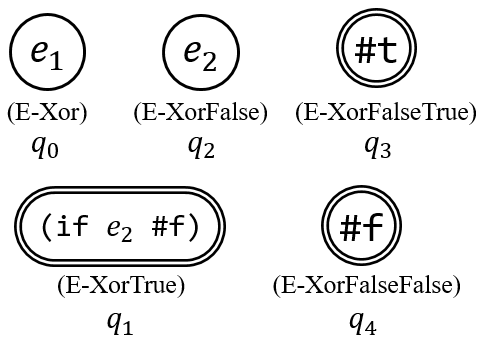
\includegraphics[scale=0.22]{images/ifa-xor-1.png}
}
\subcaptionbox{\label{fig:ifa-xor-b}}[.33\linewidth]{
    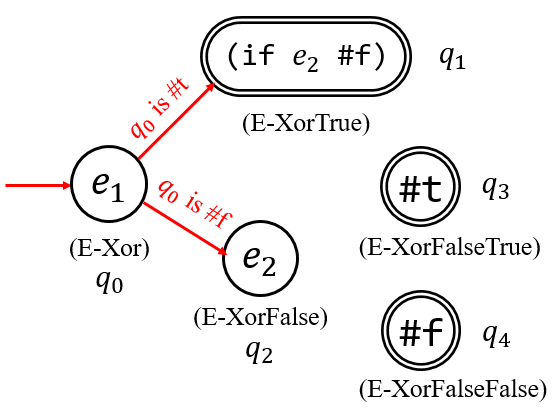
\includegraphics[scale=0.22]{images/ifa-xor-2.png}
}
\subcaptionbox{\label{fig:ifa-xor-c}}[.33\linewidth]{
    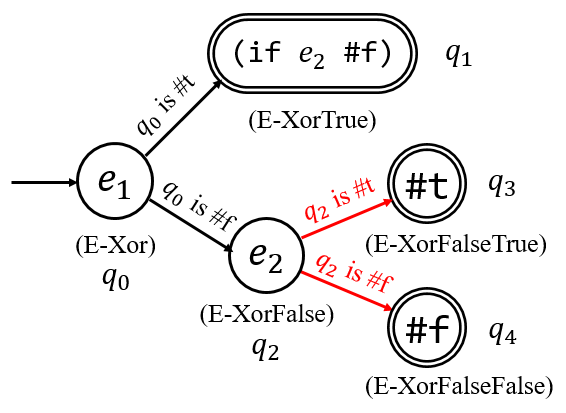
\includegraphics[scale=0.22]{images/ifa-xor-3.png}
}
\caption{IFA of \m{xor}: Constructed by evaluation rules}
\label{fig:ifa-xor}
\end{figure}

%-----------------------------
\subsubsection{IFA of \m{let}}

If a certain syntactic structure does not meet the above assumptions, it does not mean that this syntactic structure does not have an IFA. We can define its IFA according to its semantics. However, this method cannot be automated and requires users to ensure its correctness. For example, given the evaluation rules of \m{let}, we can specify the IFA of \m{let} as Figure \ref{fig:ifa-let}.

\infrule[E-Let]{e_1 \to e_1'}{\m{let}~x~e_1~e_2 \to \m{let}~x~e_1'~e_2}
\infax[E-LetSubst]{(\m{let}~x~e_1~e_2) \to e_2[e_1/x]}

\begin{figure}[t]
    \centering
    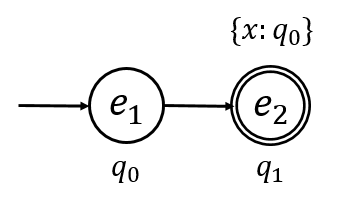
\includegraphics[scale=0.3]{images/ifa-let.png}
    \caption{IFA of \m{let}}
    \label{fig:ifa-let}
\end{figure}

In the evaluation rules of \m{let}, there is a substitution. Therefore, in IFA of \m{let}, we need symbol table to express this. When $e_2$ is evaluated or expanded, it is necessary to replace $x$ with the value of node $q_0$ in $e_2$.

%--------------------------
\subsubsection{Correctness}



%===========================================
\subsection{Convert IFA to Evaluation Rules}

Next we will try to convert IFA to evaluation rules. Because IFA can be converted into standard IFA by Theorem \ref{mythm:stdifa}, we only need to convert standard IFA into rules. Unfortunately, IFA can express some derivation methods whose evaluation rules are difficult to describe. Therefore, we also need to have stricter constraints on IFA to ensure that evaluation rules can be generated.

\begin{Asm}
\label{Asm:st}
In a standard IFA, if $q \notin F$, then the symbol table of $q$ is empty, and the expression of $q$ cannot be pattern variable.
\end{Asm}

In fact, this is a very strong assumption, which requires that only termination nodes could have substitution. Because it is difficult for us to generate a context rule for the term after substitution. \todo{\textbf{@zhichao:} We will give a counterexample containing this situation at the end.}

%------------------------
\subsubsection{Algorithm}

Similarly, we first give its algorithm, and then prove its correctness.

\begin{mythm}[Rules Can Be Constructed by Standard IFA]
\label{mythm:ifa2rule}
For each standard IFA satisfy Assumption \ref{Asm:st}, it can be converted to evaluation rules.
\end{mythm}

\begin{proof}[Proof of Theorem \ref{mythm:ifa2rule}]

Suppose that the IFA stands for the syntactic structure $H$, then we will build evaluation rules for $H$. First traverse all nodes to find the set of all terms in nodes, which is the parameters of the syntactic structure $H$ like $(\m{H}~e_1 \ldots e_n)$. Then generate evaluation rule for each node.

Begin with $q_0$, traverse the IFA. Let $q$ be $q_0$. Record the conditions by a set $T$.

Suppose that $q$ is a terminal node, the expression of $q$ is $e$ and the symbol table of $q$ is like $\{x:q_x; y:q_y; \ldots\}$. Let $e_x,e_y,\ldots$ be the expressions of $q_x, q_y, \ldots$. Add a reduction rule like

\infrule[E-Hr]{T}{(\m{H}~e_1 \ldots e_n) \to e[e_x/x][e_y/y]\ldots}

If $q$ is not a termination node, and the expression of $q$ is $e_i$, add a context rule like

\infrule[E-Hi]{e_i \to e_i' \quad T}{(\m{H}~e_1~\ldots~e_i~\ldots~e_n) \to (\m{H}~e_1~\ldots~e_i'~\ldots~e_n)}

For each condition $c$ and node $q'$ satisfying $\delta(q, c)=q'$, do the following steps separately. Replace the node in $c$ with its expression and add it to $T$. Let $q'$ be $q$. Keep doing this until $q$ is a terminal node.

\end{proof}

%----------------------------------------------------------
\subsubsection{Example: Construct Rules of \m{nand} by IFA}

Figure \ref{fig:ifa-nand-bs} is the IFA of \m{nand} which have been constructed. We can simplify it and get a standard IFA as Figure \ref{fig:ifa-nand-as}.

\begin{figure}[t]
\centering
\subcaptionbox{Before Simplification\label{fig:ifa-nand-bs}}[.45\linewidth]{
    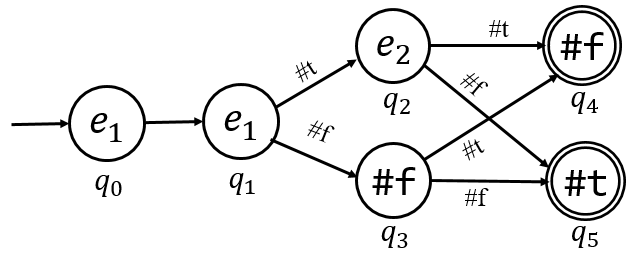
\includegraphics[scale=0.28]{images/ifa-nand-4.png}
}
\subcaptionbox{After Simplification\label{fig:ifa-nand-as}}[.45\linewidth]{
    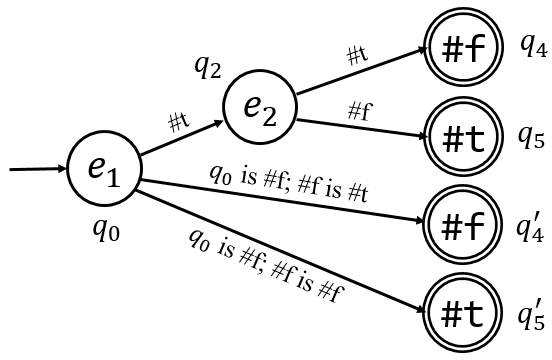
\includegraphics[scale=0.28]{images/ifa-nand.png}
}
\caption{IFA of \m{nand}}
\label{fig:ifa-nand-std}
\end{figure}

Start with $q_0$, we will get a context rule as

\infrule[E-Nand]{e_1 \to e_1'}{(\m{nand}~e_1~e_2) \to (\m{nand}~e_1'~e_2)}

We first discuss the branch of $q_2$. Add $e_1 \key{is} \m{\#t}$ to $T$. Because $q_2$ is not a terminal node, add a new context rule for $q_2$.

\infrule[E-NandTrue]{e_2 \to e_2'\quad e_1~\key{is}~\m{\#t}}{(\m{nand}~e_1~e_2) \to (\m{nand}~e_1~e_2')}

Since $q_4$ is a reduction rule, append $e_2 \key{is} \m{\#t}$ to $T$ and add a new reduction rule for $q_4$. Reduction rule for $q_5$ is similar.

\infrule[E-NandTrueTrue]{e_1~\key{is}~\m{\#t}\quad e_2~\key{is}~\m{\#t}}{(\m{nand}~e_1~e_2) \to \m{\#f}}

\infrule[E-NandTrueFalse]{e_1~\key{is}~\m{\#t}\quad e_2~\key{is}~\m{\#f}}{(\m{nand}~e_1~e_2) \to \m{\#t}}

Back to $q_0$, for $q_4'$ and $q_5'$ are also terminal nodes, we can build reduction rules for $q_4'$ and $q_5'$ in the same way.

\infrule[E-NandFalse1]{e_1~\key{is}~\m{\#f}\quad \m{\#f}~\key{is}~\m{\#t}}{(\m{nand}~e_1~e_2) \to \m{\#f}}

\infrule[E-NandFalse2]{e_1~\key{is}~\m{\#f}\quad \m{\#f}~\key{is}~\m{\#f}}{(\m{nand}~e_1~e_2) \to \m{\#t}}

We can judge that \m{\#f} is not \m{\#t}, so we can remove the rule (NandFalse1) from the rules, for it contains a condition that will never be met. At the same time, we rewrite the remaining rules into a more customary form.

\infrule[E-Nand]{e_1 \to e_1'}{(\m{nand}~e_1~e_2) \to (\m{nand}~e_1'~e_2)}
\infrule[E-NandTrue]{e_2 \to e_2'}{(\m{nand}~\m{\#t}~e_2) \to (\m{nand}~\m{\#t}~e_2')}
\infax[E-NandTrueTrue]{(\m{nand}~\m{\#t}~\m{\#t}) \to \m{\#f}}
\infax[E-NandTrueFalse]{(\m{nand}~\m{\#t}~\m{\#f}) \to \m{\#t}}
\infax[E-NandFalse]{(\m{nand}~\m{\#f}~e_2) \to \m{\#t}}

%--------------------------
\subsubsection{Correctness}

\begin{lemma}
\label{lemma:ifa2rule-correct}
For any syntactic structure \m{H}, if its standard IFA meets the above assumptions, the evaluation rules obtained according to the algorithm in Theorem \ref{mythm:ifa2rule} have the same semantics as IFA.
\end{lemma}

In other words, for any term of syntactic structure \m{H}, evaluating the term by IFA and evaluating by rule will get the same derivation sequence.

\begin{proof}[Proof of Lemma \ref{lemma:ifa2rule-correct}]
We only need to discuss that in a one-step derivation, both will get the same result.

Considering a term $e=(\m{H}~e_1 \ldots e_n)$ use rule $r$ to derive. The term $e$ must meet the condition $T$ of $r$ such as some parameters must be value or a specific value. Suppose $r$ is generated by node $q$. Then $T$ is the set of all transition conditions from $q_0$ to $q$. Therefore, the one-step derivation of this term $e$ in IFA must be located at $q$. If $r$ is a context rule for $e_i$, the expression of $q$ is $e_i$ as well, and $e_i$ of $e$ is not a value. Thus both of the one-step derivation of $e$ are one-step derivation of $e_i$. \todo{\textbf{@zhichao:} There will be no two nodes, and their conditions are exactly the same.}

Similarly, if an term can be derived in one step in IFA, then it must be able to use the corresponding rule for one-step derivation.

\end{proof}

%===========================
\subsection{Syntactic Sugar}

We can find out that although rules of \m{nand} we used when constructing the IFA included the syntactic structure of \m{if}, the final result does not. For syntactic sugar, we also deal with it with a similar idea, that is, construct the IFA of syntactic sugar, simplify it and convert it into rules. With the IFA, we can easily get the evaluation rules for syntactic sugars.

Similarly, we also need to add some constraints on syntactic sugar.

\begin{Asm}[Orderliness of Syntactic Sugar]
\label{Asm:orderliness-sugar}
The definition of each syntactic sugar can only use the syntactic structure in coreLang and the syntactic sugar that has been defined.
\end{Asm}

\begin{Def}
\label{def:ifa-sugar}
Considering the following syntactic sugar
\[
\drule{(\m{SurfHead}~x_1~\ldots~x_n)}{e},
\]
the IFA of \m{SurfHead} is defined as the IFA of syntactic structure \m{SurfHead'} whose evaluation rule is
\infax[E-SurfHead]{(\m{SurfHead'}~x_1~\ldots~x_n)\rightarrow e}

\end{Def}

%--------------------------------------------
\subsubsection{An Example of Syntactic Sugar}

Suppose that there are only \m{if} and \m{let} in our CoreLang, whose IFAs are known. Now we will build rules for syntactic sugar \m{or} and \m{sg}.

\[
\drule{\m{or}~e_1~e_2}{(\m{let}~x~e_1~(\m{if}~x~x~e_2))}
\]

\m{or} syntactic sugar only uses the syntax structure of CoreLang, which meets Assumption \ref{Asm:orderliness-sugar}. Then we will generate evaluation rules for \m{or}.

\begin{figure}[t]
    \centering
    \subcaptionbox{Rule of Definition \ref{def:ifa-sugar} \label{fig:ifa-ex-or-1}}[.31\linewidth]{
        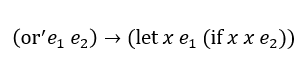
\includegraphics[scale=0.3]{images/ifa-ex-or-1.png}
    }
    \subcaptionbox{IFA generated with the algorithm of Theorem \ref{mythm:Rule2IFA} \label{fig:ifa-ex-or-2}}[.31\linewidth]{
        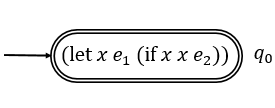
\includegraphics[scale=0.3]{images/ifa-ex-or-2.png}
    }
    \subcaptionbox{Expand syntactic structure of \m{let} \label{fig:ifa-ex-or-3}}[.31\linewidth]{
        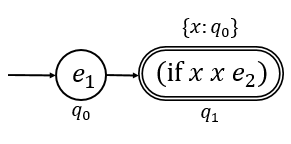
\includegraphics[scale=0.3]{images/ifa-ex-or-3.png}
    }
    \subcaptionbox{Expand syntactic structure of \m{if} \label{fig:ifa-ex-or-4}}[.31\linewidth]{
        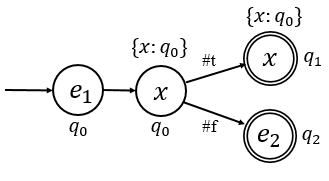
\includegraphics[scale=0.3]{images/ifa-ex-or-4.png}
    }
    \subcaptionbox{Replace \m{x} with expression according to the symbol table \label{fig:ifa-ex-or-5}}[.31\linewidth]{
        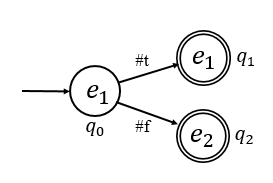
\includegraphics[scale=0.3]{images/ifa-ex-or-5.png}
    }
    \subcaptionbox{Rules generated with the algorithm of Theorem \ref{mythm:ifa2rule} \label{fig:ifa-ex-or-6}}[.31\linewidth]{
        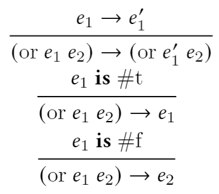
\includegraphics[scale=0.3]{images/ifa-ex-or-6.png}
    }
    \caption{Example: Syntactic Sugar of \m{or}}
    \label{fig:ifa-nand-std}
\end{figure}

The IFA of \m{or} is the same as the IFA of \m{or'} whose rule is shown in Figure \ref{fig:ifa-ex-or-1}. Therefore, we can generate an IFA according to the rule as shown in Figure \ref{fig:ifa-ex-or-2}. Next we transform IFA to make it a standard IFA, as shown in Figure \ref{fig:ifa-ex-or-3} to Figure \ref{fig:ifa-ex-or-5}. Finally, according to the structure of IFA, generate or evaluation rules, as shown in Figure \ref{fig:ifa-ex-or-6}.

% \infrule[E-Or]{e_1 \to e_1'}{(\m{or}~e_1~e_2) \to (\m{or}~e_1'~e_2)}
% \infrule[E-OrTrue]{e_1~\key{is}~\m{\#t}}{(\m{or}~e_1~e_2) \to e_1}
% \infrule[E-OrFalse]{e_1~\key{is}~\m{\#f}}{(\m{or}~e_1~e_2) \to e_2}
